\section{functionbar.h File Reference}
\label{functionbar_8h}\index{functionbar.h@{functionbar.h}}


{\tt \#include $<$qwidget.h$>$}\par
{\tt \#include $<$qpixmap.h$>$}\par
{\tt \#include \char`\"{}global\_\-define.h\char`\"{}}\par
{\tt \#include \char`\"{}enum.h\char`\"{}}\par
{\tt \#include \char`\"{}subbaralbumclock.h\char`\"{}}\par
{\tt \#include \char`\"{}subbarinternet.h\char`\"{}}\par
{\tt \#include \char`\"{}subbarplayer.h\char`\"{}}\par
{\tt \#include \char`\"{}subbarmanagement.h\char`\"{}}\par
{\tt \#include \char`\"{}subbarsetting.h\char`\"{}}\par
{\tt \#include \char`\"{}subbarclose.h\char`\"{}}\par


Include dependency graph for functionbar.h:\begin{figure}[H]
\begin{center}
\leavevmode
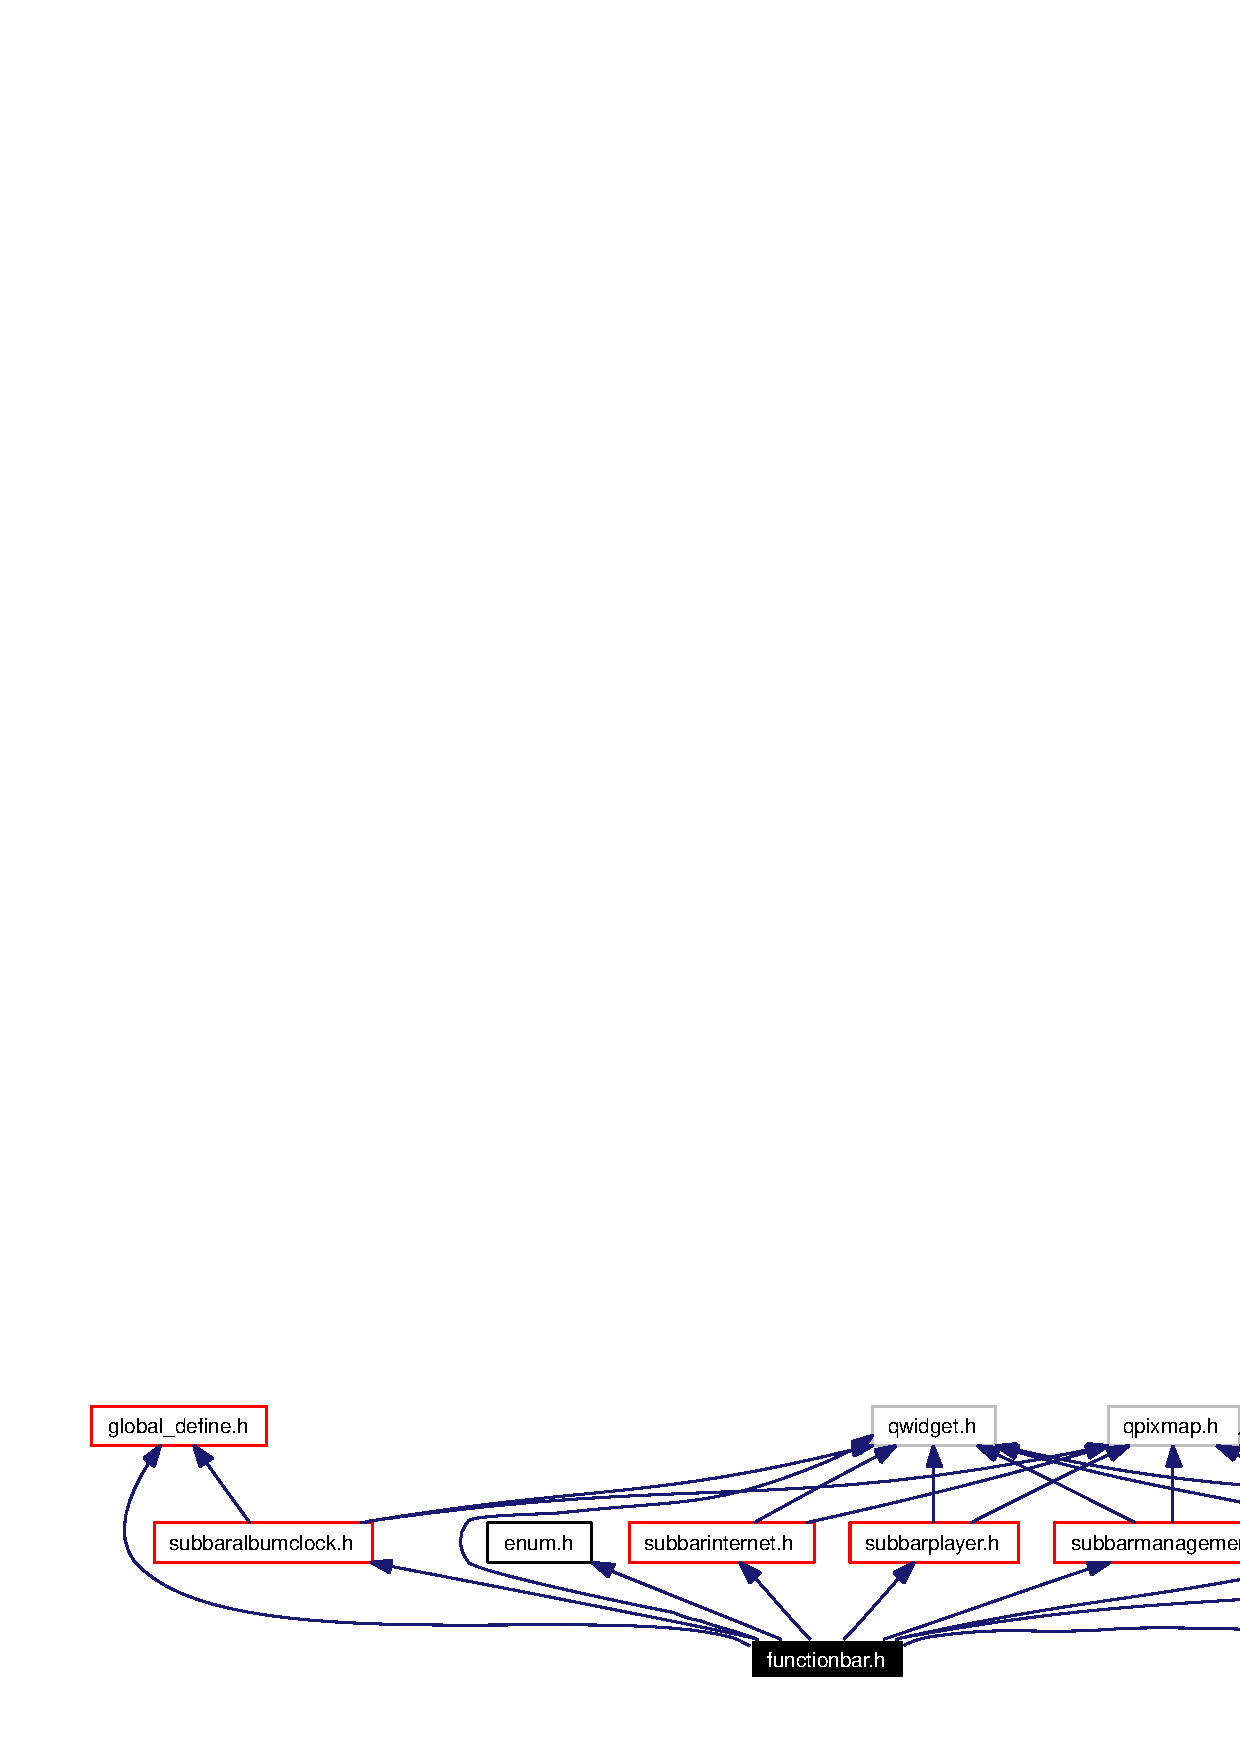
\includegraphics[width=420pt]{functionbar_8h__incl}
\end{center}
\end{figure}


This graph shows which files directly or indirectly include this file:\begin{figure}[H]
\begin{center}
\leavevmode
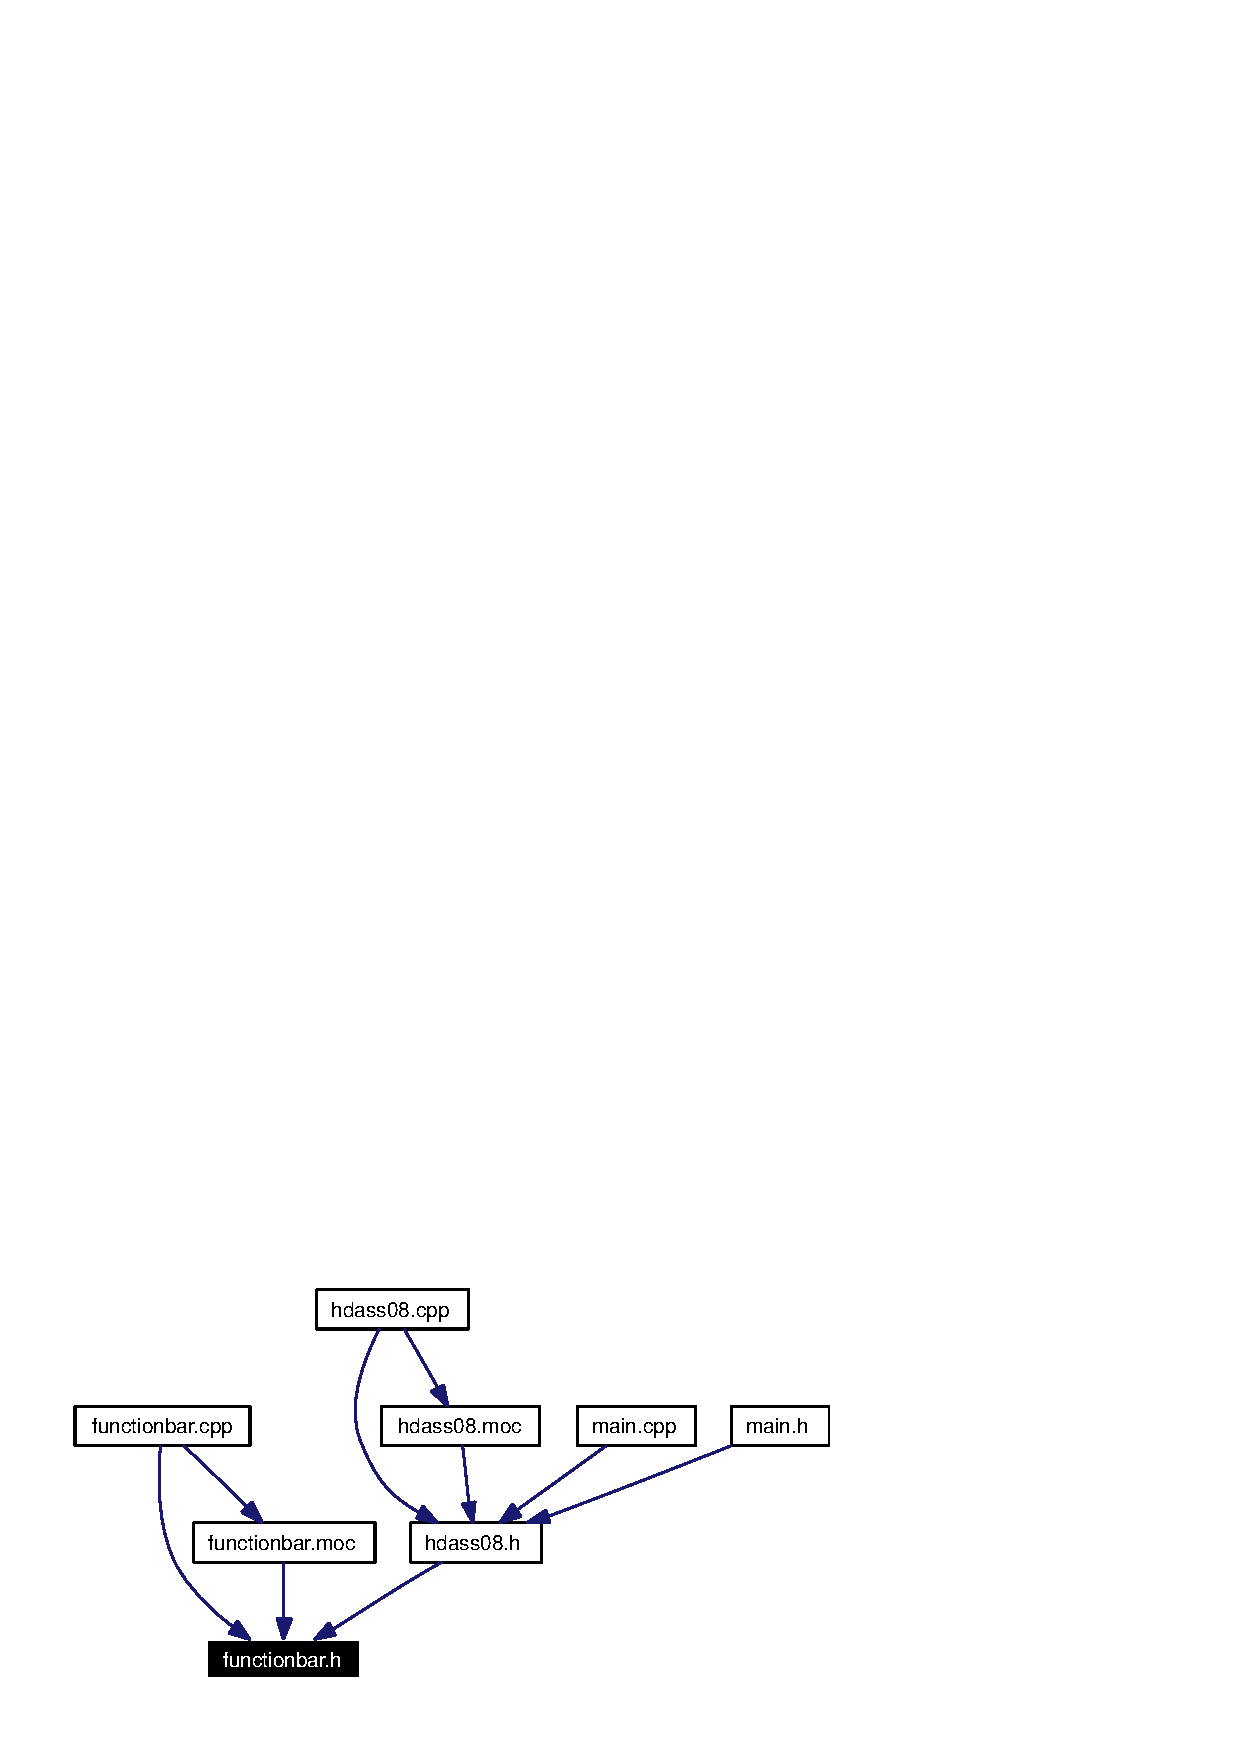
\includegraphics[width=199pt]{functionbar_8h__dep__incl}
\end{center}
\end{figure}
\subsection*{Classes}
\begin{CompactItemize}
\item 
class {\bf Function\-Bar}
\end{CompactItemize}
